\documentclass{sigkddExp}

\begin{document}
%
% --- Author Metadata here --- -- Can be completely blank or contain 'commented'
% information like this... \conferenceinfo{WOODSTOCK}{'97 El Paso, Texas USA} %
% If you happen to know the conference location etc. \CopyrightYear{2001} %
% Allows a non-default  copyright year  to be 'entered' - IF NEED BE.
% \crdata{0-12345-67-8/90/01}  % Allows non-default copyright data to be
% 'entered' - IF NEED BE. --- End of author Metadata ---

\title{Covid-19 X-ray Image Classification}
%\subtitle{[Extended Abstract]

\numberofauthors{4}

\author{\alignauthor Maneesh Kumar Singh\\
    \affaddr{University of Illinois at Urbana-Champaign}\\
    \email{mksingh4@illinois.edu}
    \alignauthor Raman Walwyn-Venugopal\\
    \affaddr{University of Illinois at Urbana-Champaign}\\
    \email{rsw2@illinois.edu}
    \alignauthor Satish Reddy Asi\\
    \affaddr{University of Illinois at Urbana-Champaign}\\
    \email{sasi2@illinois.edu}
    \alignauthor Srikanth Bharadwaz Samudrala\\
    \affaddr{University of Illinois at Urbana-Champaign}\\
    \email{sbs7@illinois.edu}
}

\date{28 March 2021}
\maketitle
\begin{abstract}
    \textbf{Objective:}
    Detecting COVID-19 using Chest X-Ray (CXR) images is becoming increasingly
    popular in deep learning research. When training deep neural networks, large
    and balanced datasets are preferred. However, since COVID-19 is new, there
    are a limited number of CXR images available which results in a challenge
    for training deep neural networks. Existing research has shown different
    approaches to address this imbalanced data issue. Two notable studies are
    FLANNEL an ensemble based network with focal loss and a patch-based
    classifier that works on segmented versions of the lung contours. We
    propose merging these two concepts together to improve performance of
    detecting COVID-19 in CXR images.

    \textbf{Materials and Methods:}
    Using segmentation networks to create masks for the lungs as a pre-processing
    step. Replace base models in FLANNEL with patch-based classifiers that take
    the image and respective mask as their input. The patch-based classifiers
    will be used as the ensemble.

    We are able to reproduce FLANNEL and base models results using the updated
    datasets. We were also able to reproduce patch-based classification using
    X-ray images. We also created a segmentation network that can produce masks
    of the lung contours for CXR images. We successfully used this segmentation
    network to produce masks of the CXR images in the updated FLANNEL datasets.

    \textbf{Results:}
    We saw improvement in metrics when training the base models and FLANNEL
    ensemble in detecting COVID-19 images. Since no parameters were changed, we
    suspect that this is due to the increase of COVID-19 images for the dataset
    in comparison to when the FLANNEL paper was written. We are in the process
    of training the patch-based classifiers to use as the base models for the
    ensemble.

    \textbf{Discussion:}
    With the success of performing segmentation on the dataset and the increased
    performance of the original base models due to the increased dataset size,
    we are hoping that this will lead to a further improvement once we finalize
    the patch-based classifiers. Our optimism is due to the patch-based
    classifiers outperforming their “global” counterparts that processed the
    whole non-segmented image.

\end{abstract}

\section{Introduction}
Coronavirus disease 2019 (COVID-19) is a contagious disease caused by severe
acute respiratory syndrome Coronavirus 2 (SARS-CoV-2). It has spread worldwide
leading to ongoing pandemic. This pandemic has ravaged the world on an
unprecedented scale. By April 2021, 141 million people have been infected with
over 3 million deaths \cite{whocovid1920-apr-21}. Chest X-Ray (CXR) is one of
the important, non-invasive clinical diagnosis tools that helps to detect
COVID-19 and other pneumonia for affected patients.

Using deep learning for X-ray classification is an ongoing research area and
recently there have been promising models proposed for COVID-19 classification.
The problem that all of these models face is an imbalance dataset due to the
limited number of COVID CXR images available.

FLANNEL is a COVID-19 CXR classification model proposed by Zhi Qiao et al.
\cite{10.1093/jamia/ocaa280} that has been shown to accurately detect COVID-19
even when trained with only 100 available COVID-19 x-ray images. There are two
core components for the FLANNEL architecture, the first is that it uses an
ensemble \cite{58871} of five independent base learners that predict the
classification of the CXR. Each of the predictions are then passed through
another ensemble network to determine the final prediction classification. The
goal of the ensemble is to increase the robustness and accuracy of the network
since each base learner should capture patterns in the images independently
\cite{combine}. The second core component for the FLANNEL is its use of the
special Focal Loss \cite{lin2018focal} function, a modification of the standard
cross-entropy loss that places a focus on the imbalance negatives by applying
down-weights to well-classified examples. Focal Loss has been known to improve
performance for imbalanced datasets.

Park et. al \cite{pmid32396075} has also created a deep learning model that has
been proven to be effective on detecting COVID-19 when trained with limited
datasets. The approach taken was to first detect lung contours of the CXR and
perform segmentation. The motivation for performing segmentation first is that
the patch based model focuses on the lung area since it’s the primary region of
interest used to perform analysis.  In general, standard biomarkers
\cite{pmid32396075} from CXR images analyzed are the following
\begin{enumerate}
    \item Lung Morphology Mean Lung Intensity
    \item Standard Deviation of Lung Intensity
    \item Cardiothoracic Ratio (CTR)
\end{enumerate}

Thus it could be observed that most of the initial diagnosis is carried out from
CXR images by concentrating the lung area, that is our motivation to adopt this
thought to have the patched method integrate with Flannel approach. We also find
by doing this it makes the model less susceptible to noise happening outside the
lung region. After the lungs have been segmented, patch-based classification is
performed. Patch-based classification involves selecting random crops or patches
across the image for a set number of times and then performing classification on
each patch. Afterwards, the final prediction of the image is made by majority
voting based on the prediction of each patch. From the graphs provided in the
paper \cite{pmid32396075} by Park and Ye, it is clear that the patch-based
classification outperformed the models that used the whole image for a limited
train set data. As we have an imbalanced dataset with limited COVID 19 CXR
images, we are optimistic that utilizing patch-based classification models for
the FLANNEL ensemble with the combination of focal loss optimization would
result in a performance improvement.

Our goal is to take the novel ideas of each approach listed above with the goal
of improving performance. To accomplish this we will make modifications to the
existing FLANNEL architecture by first pre-processing the CXR images by
performing segmentation of the lung contours. Afterwards, we will then update
the independent base learners in the ensemble to be patch-based classifiers. We
call this new architecture “Patched FLANNEL”. The network structure is shown in
Figure \ref{fig:improve} and similar to FLANNEL consists of two stage approach.


\section{Method}

The primary objective was to improve the detection of COVID-19 in CXR images
with a multi-classifier model that can detect Normal, Pneumonia Viral, Pneumonia
Bacteria and COVID-19. The baseline we will be comparing against is the original
FLANNEL architecture. We used the same datasets that were used in the FLANNEL
paper, the COVID Chest X-ray Dataset \cite{cohen2020covidProspective} from
\href{https://github.com/ieee8023/covid-chestxray-dataset}{GitHub} and the
\href{https://www.kaggle.com/paultimothymooney/chest-xray-pneumonia}{Kaggle
    Chest X-ray} images dataset. Similar to the FLANNEL paper, we also restricted
the types of images used to anteroposterior (AP) or posteroanterior (PA). The
restricted images were then labelled into one of four categories; COVID-19,
Viral Pneumonia, Bacterial Pneumonia and Normal.

The first major data pre-processing step that we performed on our dataset was
segmentation. In order to accomplish this, we recreated the same segmentation
network that Park et al. used for their patch-based classification;
FC-DenseNet103 \cite{DBLP:journals/corr/JegouDVRB16}. We trained the
FC-DenseNet103 model using PyTroch to produce a mask of the lung contours of a
CXR image. The datasets that were used to train the segmentation network were
the Japanese Society of Radiological Technology (JSRT)
\href{http://db.jsrt.or.jp/eng.php}{dataset} which contained 247 PA CXR images
and the Segmentation in Chest Radiographs (SCR)
\href{https://www.isi.uu.nl/Research/Databases/SCR/}{database} which contains
segmentation masks for the CXR images from the JSRT dataset. The JSRT/SCR
dataset were randomly split where 80\% of images were used for training and 20\%
were used for validation; this resulted in 197 images being used for training
and 50 images being used for validation for the JSRT dataset as shown in Table
\ref{table:segdata}. Since CXR images from different data sources will come in a
wide variety of formats, the JSRT dataset was pre-processed by performing data
type casting to float32, histogram equalization to adjust the contrast, gamma
correction to adjust brightness and standardizing the image size by resizing it
to 256x256. During training, the network parameters were initialized with a
random distribution and the Adam optimizer was used with an initial learning
rate of 0.0001. The learning rate was decreased by a factor of 10 when there was
no improvement in the loss. The Jaccard Index (JI) was used to evaluate the
model during training since we were comparing the similarity of the mask
produced by the network to the mask provided in the SCR dataset. An early
stopping strategy was used based on the validation performance to prevent the
model from overfitting.

We then applied the trained FC-DenseNet103 segmentation model on the AP and PA
CXR images from the Covid Chest X-ray and Kaggle X-ray datasets, this resulted
in producing a mask for the lung contours for each of the images. We then split
the segmented dataset using a train-test ratio of 4:1 to randomly generate train
test splits. To ensure reporting accurate performance on the base models, we
used five fold cross validation while training. The detailed statistics are
shown in Table \ref{table:datastats}.

The next improvement that we produced was creating patch-based classifiers.
Similar to the original global base models in FLANNEL, the patch base models
used were pre-trained from ImageNet to account for the small size of the
dataset. The pre-processed images were first resized to 1024x1024 to be as close
to the original pixel distribution. The masks generated from the FC-DenseNet103
segmentation model were also upsampled to 1024x1024 to match the new CXR image
size.The resized images were then masked with the lung-contours and passed as
input to the patch-based classifier. The patch-based classifier then produced k
number crops/patches of size 224x224 from the CXR. To limit patches outside the
lung area, the random points were forced to be within the lungs and the random
point was used as the center of the patch. During inference, the k should be
large enough to ensure that the lung pixels are covered multiple times. Each
patch is then fed into a network to produce a prediction. The confidence score
was calculated for each category by calculating the percentage of predictions
for each class based on the k patches. The optimization algorithm used during
training was the Adam optimizer with a learning rate of 0.00001. An early
stopping strategy based on validation performance was applied and a weight decay
and L1 regularization were used to prevent overfitting. The best model is
selected among 200 epochs training. The overall algorithm is shown in Algorithm
\ref{algo:flannel-improved}.

\setlength{\algomargin}{0pt}
\begin{algorithm}
    \SetAlgoNoLine
    \DontPrintSemicolon
    \SetKwProg{Input}{Input:}{}{}
    \SetKwBlock{AlgBlock}{}{}
    \SetKwInOut{Input}{Input}
    \SetKwInOut{StageOne}{Stage 1}
    \SetKwInOut{StageTwo}{Stage 2}
    \SetKwFor{ForE}{For each}{do}{End For}
    \Input{\;
        X-ray Images, Class Labels\;
        Segmentation Model\;
        Base Models \{$Learner_1, Learner_2, …, Learner_n$\}\;
        \emph{(Define B as batch size)}\;
        \emph{(Define K patch count)}\;
    }

    \StageOne{\;
        Run segmentation network on the dataset to generate masks for each CXR image.\;
    }
    \StageTwo{\;
        \ForE{batch of images from input images and labels}{
            1. Fetch the segmented mask and image.\;
            2. Resize the CXR image to 1024x1024.\;
            3. Upscale the mask to 1024x1024.\;
            4. Separate image into random k patches.\;
            5. Pass random k-patches to base models.\;
            6. Perform majority voting to get get confidence scores/prediction values from each base model.\;
            7. Get prediction values from all Base Models.\;
            $P_i = Learner_i(X) \in R^{B\times 4}$, where i = 1,...n\;
            8. Get Learner weights.\;
            $W=NeuralWeightModule([P_i, i=1,..,n]) \in R^{B\times 5}$\;
            9. Linear Combination for Prediction\;
            $\hat{Y}=Softmax(\sum_{i=1}^{n} W_i P_i) \in R^{B \times 4}$ (where $W_i$ represents i-th column of $W$)\;
            10. Loss = $FocalLoss(\hat{Y}, Y)$\;
            11. Back-propagate on Loss and update parameters
        }
    }

    \caption{FLANNEL with patch-by-patch Training}
    \label{algo:flannel-improved}
\end{algorithm}

\subsection{Considerations}
Here are our considerations discussed below -
\begin{itemize}
    \item The pretrained model for segmentation (FC-Densenet103) will perform
          well on the datasets used in FLANNEL \cite{10.1093/jamia/ocaa280} paper.
    \item The number of patches(K) to be 100 to start with, will be fine tuned
          after evaluating the results.
    \item The patch image size will be chosen as 224X224 initially and will be
          fine tuned after evaluating the results.
\end{itemize}


\begin{figure*}[h]
    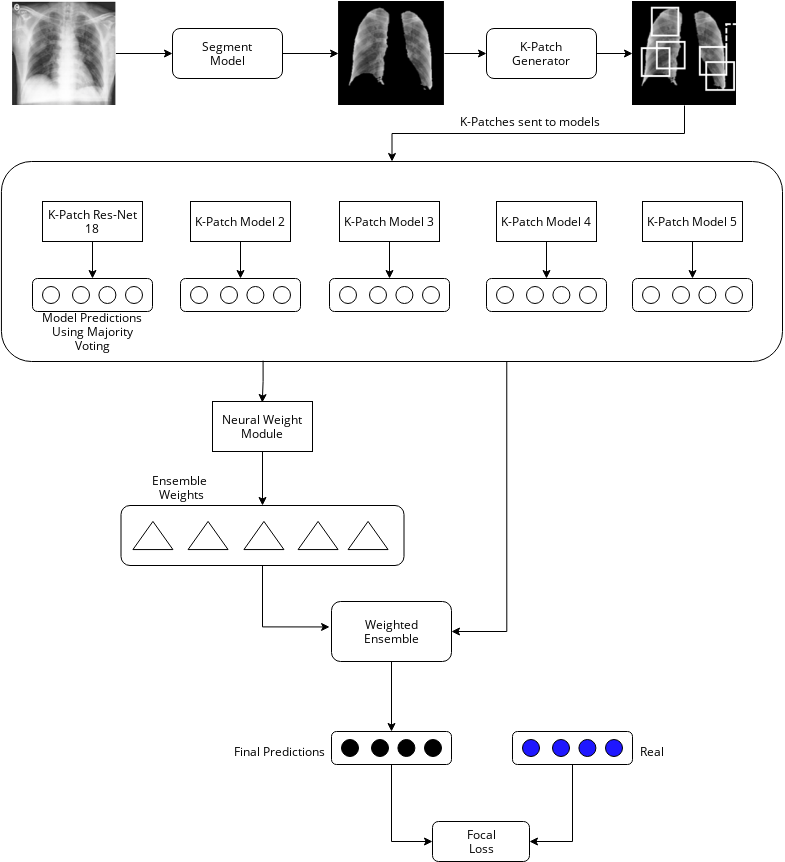
\includegraphics[width=0.8\textwidth]{../doc/images/FLANNEL-IMPROVED.png}
    \caption{FLANNEL Improvement}
    \label{fig:improve}
\end{figure*}



\begin{table}
    \caption{FC\-DenseNet103 Segmentation Training \& Validation Dataset}
    \label{table:segdata}
    \begin{tabular}{ll} \hline
        Dataset    & Number of images \\ \hline
        Training   & 197              \\
        Validation & 50               \\
        \hline
    \end{tabular}

\end{table}

\begin{table*}
    \centering
    \caption{Experimental data description}
    \label{table:datastats}
    \begin{tabular}{llrrrrr} \hline
        Source                                 &           & Total  & COVID-19 &
        Viral                                  & Bacterial & Normal              \\ \hline
        \multirow{2}{*}{} Original data        & CCX data  & 554    & 478      &
        16                                     & 42        & 18                  \\
                                               & KCX data  & 5856   & 0        &
        1493                                   & 2780      & 1583                \\
        \hline
        \multirow{2}{*}{} View Distribution    & AP view   & 6163   & 282      &
        1501                                   & 2789      & 1591                \\
                                               & PA view   & 247    & 196      &
        8                                      & 33        & 10                  \\ \hline
        \multirow{3}{*}{} Training/test splits & Training  & 5127   & 378      &
        1509                                   & 2291      & 1288                \\
                                               & Testing   & 1283   & 100      &
        339                                    & 531       & 313                 \\
                                               & Total     & 6410   & 478      &
        1509                                   & 2822      & 1601                \\
        \hline
    \end{tabular}\par
    \bigskip
    AP: anteroposterior; CCX: COVID Chest X-ray; COVID-19: coronavirus disease
    2019; KCX: Kaggle Chest X-ray; PA: posteroanterior.
\end{table*}



\begin{table*}
    \centering
    \caption{Performance comparison on F1 score: Class-specific F1 score is calculated using 1 class vs the rest strategy}
    \label{table:resultstats}
    \begin{tabular}{ lccccc } \hline
                         & COVID-19      & Pneumonia virus & Pneumonia bacteria &
        Normal           & Macro-F1                                               \\ \hline

        Densenet161      & 0.7694 (0.03) & 0.5901 (0.05)   & 0.8030 (0.01)      &
        0.8875 (0.02)    & 0.7625 (0.02)                                          \\
        InceptionV3      & 0.8938 (0.01) & 0.6413 (0.03)   & 0.8112 (0.02)      &
        0.9015 (0.03)    & 0.8120 (0.02)                                          \\
        Resnet152        & 0.8302 (0.02) & 0.6218 (0.02)   & 0.8046 (0.01)      &
        0.9080 (0.00)    & 0.7911 (0.01)                                          \\
        ResNeXt101       & 0.8197 (0.03) & 0.6151 (0.04)   & 0.8016 (0.01)      &
        0.9046 (0.01)    & 0.7852 (0.02)                                          \\
        Vgg19\_bn        & 0.8753 (0.02) & 0.6023 (0.01)   & 0.8016 (0.01)      &
        0.8950 (0.00)    & 0.7936 (0.00)                                          \\
        FLANNEL\_OldData & 0.8168 (0.03) & 0.6063 (0.02)   & 0.8267 (0.00)      &
        0.9144 (0.01)    & 0.7910 (0.01)                                          \\
        FLANNEL          & 0.9239 (0.01) & 0.6675 (0.02)   & 0.8306 (0.01)      &
        0.9322 (0.00)    & 0.8385 (0.01)                                          \\ \hline
    \end{tabular}\par
    \bigskip
    The values in parentheses are the standard deviations.
\end{table*}

\section{Results}

We chose 5 base learners for FLANNEL framework, Densenet161, InceptionV3,
Resnet152, ResneXt101 and Vgg19\_bn. These models were fine-tuned using default
parameter values, settings and by using the Adam optimizer. We compared FLANNEL
with these 5 base learners of the framework.

We are planning to create and train patch-based versions of the base learners
that will use the masked version of the same images from the dataset. We will
then re-run the FLANNEL with the patch-based learners and compare performance.
In addition to the improvements, we are  also planning to compare 2 recent
COVID-19 deep learning models, COVID-Net \cite{wang2020covidnet} and AI-COVID
\cite{pmid32339081}.


\subsection{Evaluation strategy}
Our main goal is to study the detection of COVID-19 among different respiratory
x-ray images. We first measured the overall accuracy and precision of all 4
classes of x-ray images (COVID-19 viral pneumonia, non-COVID-19 viral pneumonia,
bacterial pneumonia and normal images).

For each class of image, we record precision and recall values for each fold.
We calculate F1-score for each fold and then average them to calculate the mean
F1 score.

We are evaluating the global base learners independently, the global ensemble,
the patch-based learners independently and the patch-based ensemble.

\subsection{Implementation Details}
The FC-DenseNet103 segmentation model was implemented in PyTorch and trained on
a NVIDIA 1080 GPU.

FLANNEL with patch-based classification are implemented in PyTorch and are
trained on 4 different Amazon Web Services Elastic Compute Cloud virtual
machines each featuring a single NVIDIA Tesla V100 GPU. The base models
are fine tuned using pre-trained models. The data are
augmented with random flips, crops and scaling during the fine tuning process.

After the base models are trained, FLANNEL is trained by passing in the
concatenated output layers of the base models as the input features.

\subsection{Experimental Results}
\subsubsection{Segmentation Training}
Training the Segmentation Network on the JSRT/SCR dataset had a Jaccard Index
(JI) score of 93.39\% for creating the lung contour masks. The figure \ref{fig:segtrain}
shows the mask creation and applying the mask on the image.

\begin{figure}[h]
    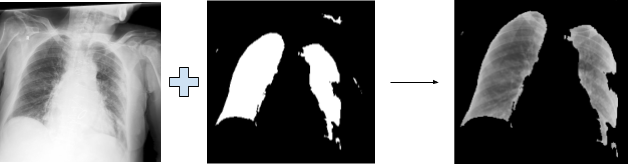
\includegraphics[width=8cm]{../doc/images/segmentation_training.png}
    \caption{Segmentation Training}
    \label{fig:segtrain}
\end{figure}

\subsubsection{FLANNEL}

When reproducing the FLANNEL paper we used the same base models;  Densenet161,
InceptionV3, Resnet152, ResneXt101 and Vgg19\_bn. These models were fine-tuned
using the default parameter settings and by using the Adam optimizer. We
compared FLANNEL ensemble performance with the independent performance for each
of the base models. The overall accuracy is not the appropriate measure for
evaluation of the model due to the fact that our dataset is imbalanced in favor
of non-COVID-19 related pneumonia images. With this imbalance, even a
significant increase in COVID-19 detection performance will not affect overall
accuracy much. So, we leaned towards F1 score for COVID-19 vs the rest,
comparing different models. As shown in the figure \ref{fig:f1score}, clearly
FLANNEL outperformed the other state-of-the-art models in detecting COVID-19
cases.

In Table \ref{table:resultstats}, we also show F1-score for each classification
and macro F1-score for all classes. In Table \ref{table:resultstats}, we can see
FLANNEL performed better than base models. We also see with improved data FLANNEL
scores are better than when run with old dataset containing only 100 COVID-19 images
\cite{10.1093/jamia/ocaa280}.


\begin{figure}[H]
    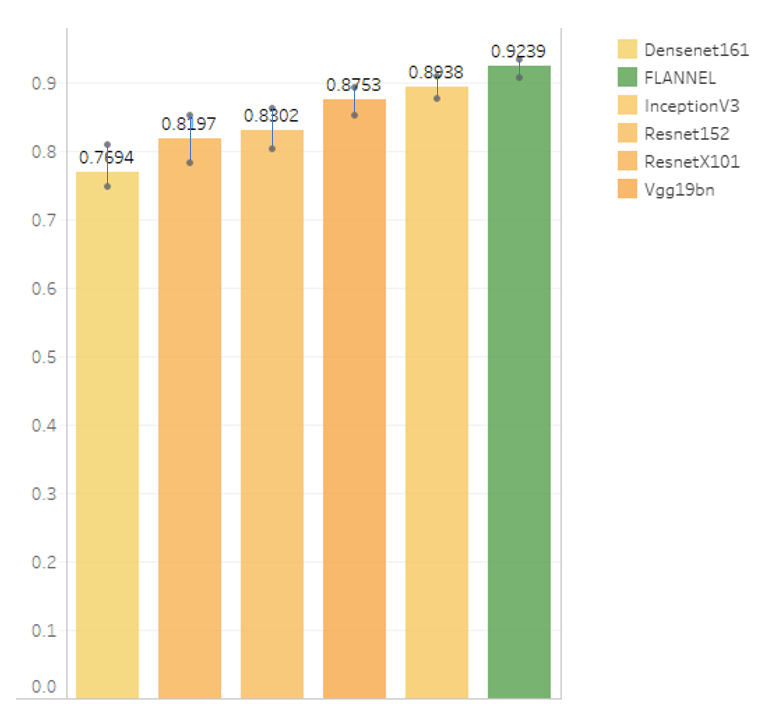
\includegraphics[width=8cm]{../doc/images/F1Score_vs_rest.png}
    \caption{FLANNEL Improvement}
    \label{fig:f1score}
\end{figure}


We also provided the visual description of FLANNEL performance, via confusion
matrix as shown in figure \ref{fig:cfmatrix}. As the matrix depicts, the cases
predicted as pneumonia are mainly from the GroundTruth pneumonia-related cases
and COVID-19 identification, FLANNEL has higher precision and recall than the
other 2 types of pneumonia. This proves FLANNEL can distinguish pneumonia images
from normal images and differentiate chest x-ray images of COVID-19 against
other pneumonia images.

\begin{figure}[h]
    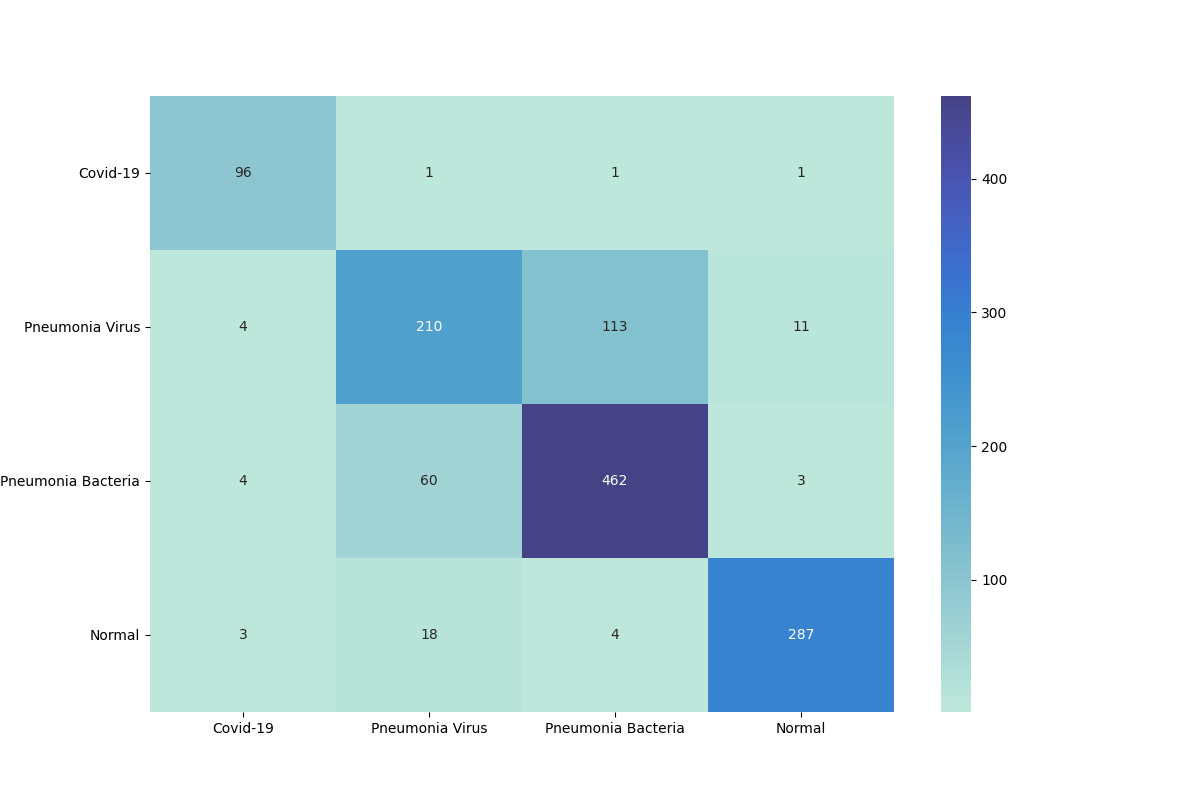
\includegraphics[width=8cm]{../doc/images/confusion_matrix.png}
    \caption{Confusion Matrix}
    \label{fig:cfmatrix}
\end{figure}

\section{Conclusion}
As we are making progress, we have run the base models and FLANNEL on the new
dataset. With the improved distribution of COVID-19 data we see FLANNEL
outperforms the metrics as seen in the base flannel paper. We completed the
Segmentation training and are able to feed that to base models. We still need to
update the FLANNEL ensemble with patch-based models and compare the performance
against the original FLANNEL. In addition to measuring classification
performance, we will also measure timing performance to note how much of an
impact the patch-based classification technique has on runtime.

\section{Acknowledgement}
GitHub source code for both FLANNEL and Patch-by-Patch classification
\cite{pmid32396075} paper are used as baseline for this improvement.
\begin{itemize}
    \item \href{https://github.com/qxiaobu/FLANNEL}{FLANNEL GitHub Repository}
    \item \href{https://github.com/jongcye/Deep-Learning-COVID-19-on-CXR-using-Limited-Training-Data-Sets}
          {Patch-by-Patch classification}
\end{itemize}



\clearpage
%
% The following two commands are all you need in the initial runs of your .tex
% file to produce the bibliography for the citations in your paper.
\bibliographystyle{abbrv}
\bibliography{covid19}  % sigproc.bib is the name of the Bibliography in this

\end{document}
